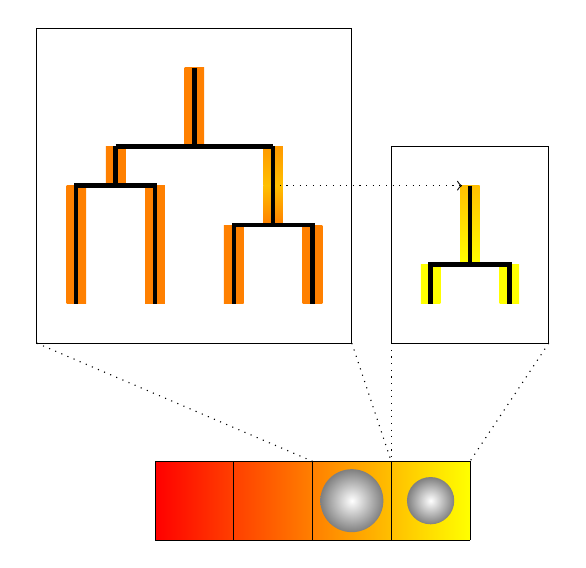
\begin{tikzpicture} 
  % Patch gradients
  \shade[left color=red,right color=yellow] (0,0) rectangle (4,1);
  % Species gradients
  \shade[inner color=white,outer color=gray] (2.5,0.5) circle (0.4 cm);
  \shade[inner color=white,outer color=gray] (3.5,0.5) circle (0.3 cm);
  % Grids
  \draw[step=1cm,black,very thin] (0,0) grid (4,1); 
  % Shade underneath left phylogeny
  \shade[top color=red!50!yellow,bottom color=red!50!yellow] (0.5-0.124,6.0) rectangle (0.5+0.124,5.0);
  \shade[top color=red!50!yellow,bottom color=red!50!yellow] (-0.5-0.124,5.0) rectangle (-0.5+0.124,4.5);
  \shade[top color=red!40!yellow,bottom color=red!25!yellow] ( 1.5-0.124,5.0) rectangle ( 1.5+0.124,4.5); % Colonization
  \shade[top color=red!25!yellow,bottom color=red!50!yellow] ( 1.5-0.124,4.5) rectangle ( 1.5+0.124,4.0); % Colonization

  \shade[top color=red!50!yellow,bottom color=red!50!yellow] (-1.0-0.124,4.5) rectangle (-1.0+0.124,3.0);
  \shade[top color=red!50!yellow,bottom color=red!50!yellow] ( 0.0-0.124,4.5) rectangle ( 0.0+0.124,3.0);
  \shade[top color=red!50!yellow,bottom color=red!50!yellow] ( 1.0-0.124,4.0) rectangle ( 1.0+0.124,3.0);
  \shade[top color=red!50!yellow,bottom color=red!50!yellow] ( 2.0-0.124,4.0) rectangle ( 2.0+0.124,3.0);
  % Left species phylogeny
  \draw[] (-1.5,2.5) rectangle (2.5,6.5); 
  \draw[ultra thick] ( 0.5,6.0) node {} -- ( 0.5,5.0) node {}; 
  \draw[ultra thick] (-0.5,5.0) node {} -- ( 1.5,5.0) node {}; 
  \draw[ultra thick] (-0.5,5.0) node {} -- (-0.5,4.5) node {}; 
  \draw[ultra thick] ( 1.5,5.0) node {} -- ( 1.5,4.0) node {}; 
  \draw[ultra thick] (-1.0,3.0) node {} -- (-1.0,4.5) node {} -- ( 0.0,4.5) node {} -- ( 0.0,3.0) node {}; 
  \draw[ultra thick] ( 1.0,3.0) node {} -- ( 1.0,4.0) node {} -- ( 2.0,4.0) node {} -- ( 2.0,3.0) node {}; 
  % Shade underneath right phylogeny
  \shade[top color=red!25!yellow,bottom color=red!00!yellow]  (4.0-0.124,4.5) rectangle (4.0+0.124,3.5);
  \shade[top color=red!00!yellow,bottom color=red!00!yellow]  (3.5-0.124,3.5) rectangle (3.5+0.124,3.0);
  \shade[top color=red!00!yellow,bottom color=red!00!yellow]  (4.5-0.124,3.5) rectangle (4.5+0.124,3.0);
  % Right species phylogeny
  \draw[] ( 3.0,2.5) rectangle (5.0,5.0); 
  \draw[ultra thick] ( 4.0,4.5) node {} -- ( 4.0,3.5) node {}; 
  \draw[ultra thick] ( 3.5,3.0) node {} -- ( 3.5,3.5) node {} -- ( 4.5,3.5) node {} -- ( 4.5,3.0) node {}; 
  % Colonization line
  \draw[dotted,->] ( 1.5,4.5) node {} -- (4.0-0.1,4.5) node {}; 
  % Zoomers
  \draw[dotted] (-1.5,2.5) node {} -- (2,1) node {}; 
  \draw[dotted] ( 2.5,2.5) node {} -- (3,1) node {}; 
  \draw[dotted] ( 3.0,2.5) node {} -- (3,1) node {}; 
  \draw[dotted] ( 5.0,2.5) node {} -- (4,1) node {}; 
  
\end{tikzpicture}